\documentclass[main.tex]{subfiles}
\begin{document}
\section{Results}

The results of an Otii measurement are depicted in Figure \ref{fig:csharp-default1}. The figure shows power draw measurements from the first C\# experiment iteration with default optimizations, with a power draw sample rate of 10,000 per second.

\begin{figure*}[]
    \centering
    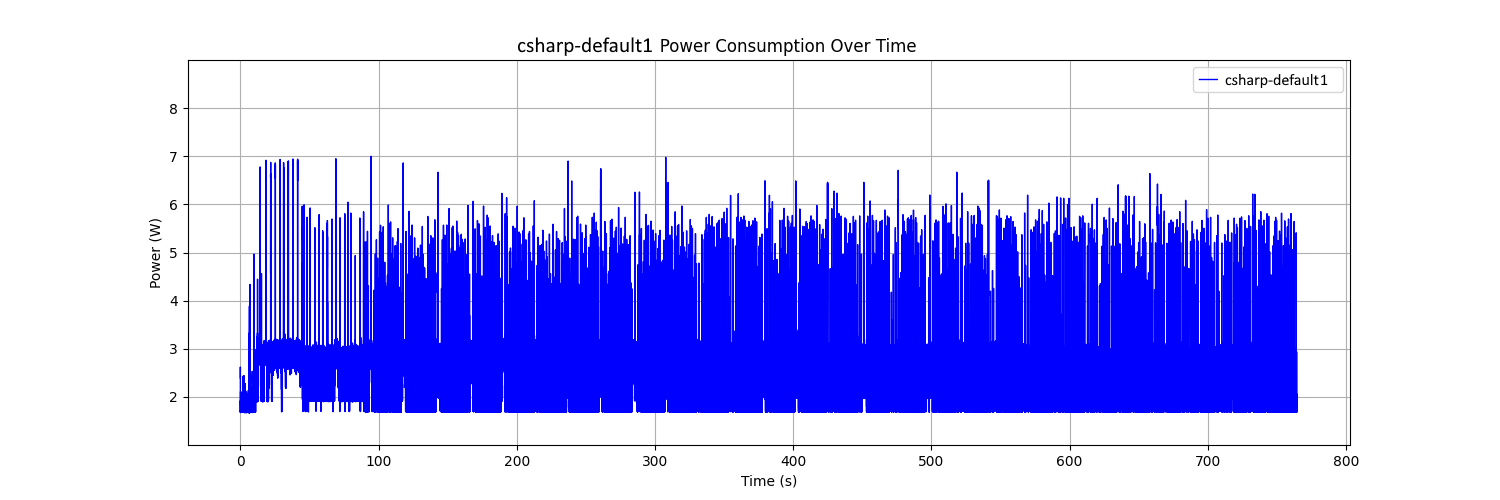
\includegraphics[width=\linewidth]{media/results/csharp-default1.png}
    \caption{Power draw of the first experiment iteration for csharp-default}
    \label{fig:csharp-default1}
\end{figure*}

The raw measurements from all experiment iterations can be found in the replication kit \cite{replication-kit-Karlsen_Landsgaard_Offenberg_Pedersen_2025}.

To better understand the energy consumption of each experiment iteration, we focus on the energy consumed per run, measured in Joules (J). The Otii provides the power draw, measured in Watts (W), which reflects the amount of power used at a specific moment. The iteration's execution time is measured in seconds (s) and reflects the time the execution took. Energy consumption combines the magnitude of power and execution time into a single metric, which is calculated as:

\[
\text{Energy (J)} = \text{Power (W)} \times \text{Execution time (s)}
\]

The power used for the calculation is the average power draw during the experiment iteration.

By combining power draw and execution time into a single value for energy consumption, we can compare iterations effectively. This also helps account for spikes in power draw during a run. For example, a short run that draws a lot of power and a long run that draws less power could use the same amount of energy. 

\begin{figure*}[]
    \centering
    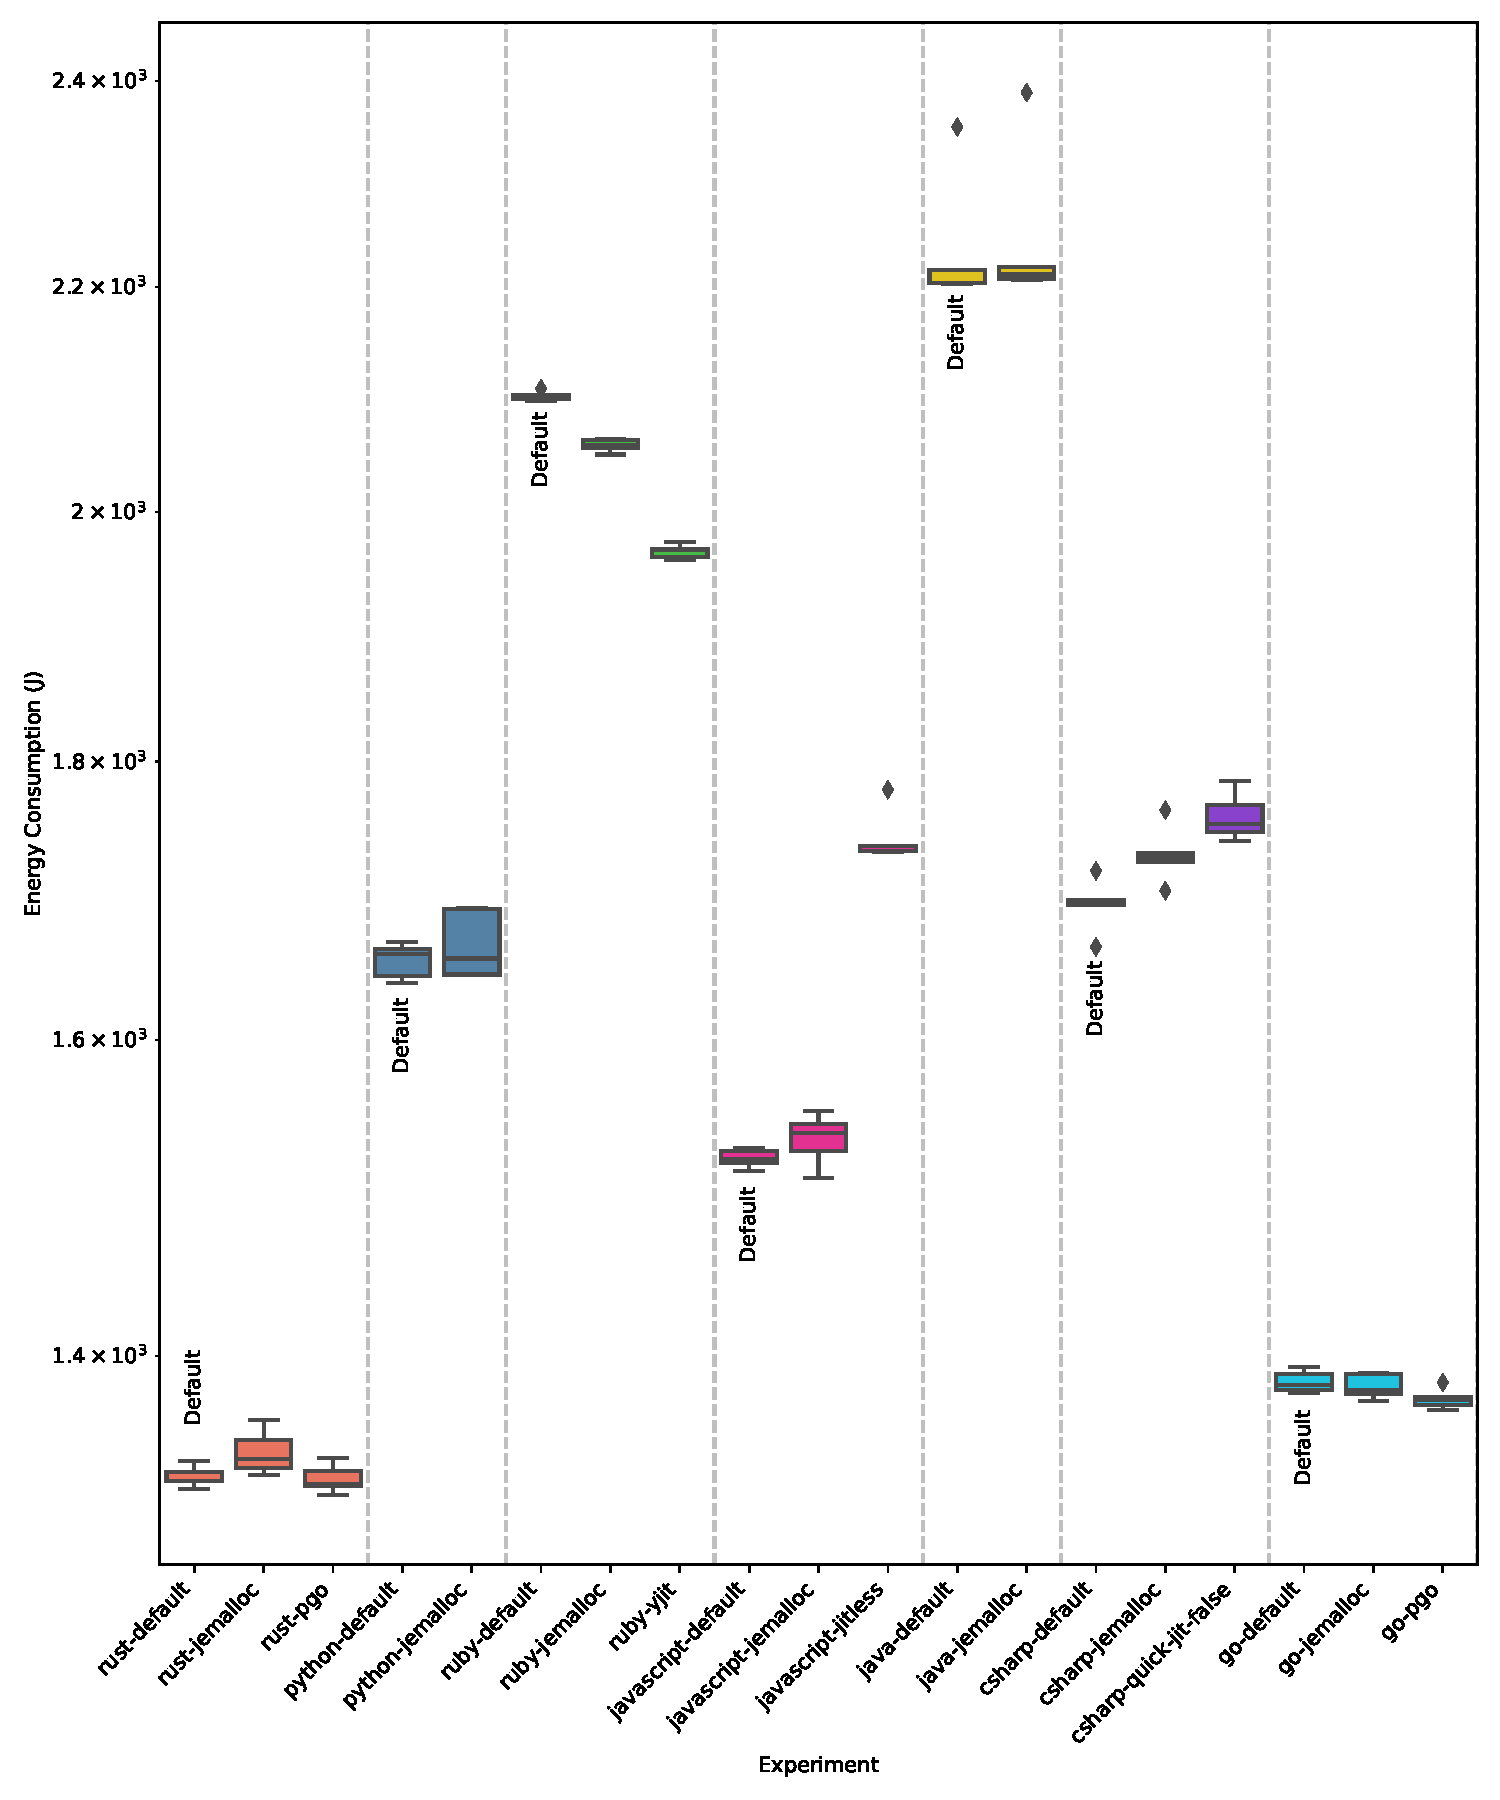
\includegraphics[scale=0.7]{media/results/boxplot.pdf}
    \caption{Boxplot of energy consumption for each experiment. Note, the y-axis spans from 1,300 to 2,400 J, and the x-axis shows each experiment}
    \label{fig:boxplot}
\end{figure*}

Figure \ref{fig:boxplot} depicts the energy consumption of all experiments grouped by implementations, with each experiment containing five experiment iterations. The y-axis uses a logarithmic scale to represent the span in energy consumption across the measurement groups, and the energy consumption ranges from approximately 1,300 J to 2,400 J.

The Go and Rust implementations show the lowest energy consumption, with values between 1,300 J and 1,400 J. Their performance is stable, showing minimal variation across iterations and experiments. 

The Java and Ruby implementations range between 1,950 J and 2,400 J, making them the most energy-intensive among the implementations. The Ruby implementation consumes less energy in the non-default experiments, demonstrating that the energy consumption can be lowered through optimizations alone. 

\subfile{../media/tables/results2}

In Table \ref{table:table-results}, each implementation has a default experiment, indicating no optimizations. These are followed by one or more rows showing different optimizations. Each entry represents the average of five experiment iterations.

Each experiment is compared against the default configuration, with the  $\Delta$ column indicating the change for each metric, including an arrow to summarize an increase (▲) or decrease (▼). Before calculating the change, all values are rounded to two decimal places to provide a clearer overview for comparing the results.

The percentage change is calculated as:

\[
\Delta E = \left( \frac{E_{\text{optimization}} - E_{\text{default}}}{E_{\text{default}}} \right) \times 100
\]

\[
\Delta P = \left( \frac{P_{\text{optimization}} - P_{\text{default}}}{P_{\text{default}}} \right) \times 100
\]

\[
\Delta t = \left( \frac{t_{\text{optimization}} - t_{\text{default}}}{t_{\text{default}}} \right) \times 100
\]

% \vspace{5mm}
\textit{Example of calculating energy change for Rust jemalloc:
}
\begin{align*}
E_{\text{default}} &= 1331.3863~\text{J} \\
E_{\text{jemalloc}} &= 1344.1615~\text{J} \\
\text{$\Delta E_{\text{jemalloc}}$} &= \left( \frac{1344.1615 - 1331.3863}{1331.3863} \right) \times 100 \approx 0.96\%
\end{align*}

% \vspace{5mm}

\subsection{Temperature}
Before and after each experiment iteration, the temperature of the Web Server is collected. Across all iterations, our pre-experiment temperatures range from 42.36°C to 46.74°C, and our post-experiment temperatures range from 43.33°C to 50.63°C. Specific data points can be found in Appendix \ref{sec:temperature-readings}.
\end{document}